\documentclass[aspectratio=169]{beamer}
\usepackage[utf8]{inputenc}
\usepackage{utopia} %font utopia imported
\usetheme{Madrid}
\usecolortheme{default}

%Information to be included in the title page:
\title{Cours d'introduction à la chimie quantique}

\subtitle{Chapitre 3 : Système simple\\Partie 2 :Oscillateur harmonique}
\author{François Dion}
%\institute{Overleaf}
\date{2020}




%\logo{\includegraphics[height=1.5cm]{lion-logo.jpg}}

%End of title page configuration block
%------------------------------------------------------------



%------------------------------------------------------------
%The next block of commands puts the table of contents at the 
%beginning of each section and highlights the current section:

%\AtBeginSection[]
%{
  %\begin{frame}
    %\frametitle{Table of Contents}
    %\tableofcontents[currentsection]
  %\end{frame}
%}
%------------------------------------------------------------


\begin{document}

%The next statement creates the title page.
\frame{\titlepage}


%---------------------------------------------------------
%This block of code is for the table of contents after
%the title page
%\begin{frame}
%\frametitle{Table of Contents}
%\tableofcontents
%\end{frame}
%---------------------------------------------------------


\section{Le potentiel}
\begin{frame}
\frametitle{Le potentiel}
\begin{columns}
\column{0.5\textwidth}
Le potentiel considéré est le cas où:
%|x| = \begin{cases} x &\text{if }x \ge 0 \\ -x &\text{if }x < 0 \end{cases}
%\begin{equation}
%\begin{eqnarray}
%\begin{eqnarray*}
%V(x) &=& 


\begin{equation} \tag{1}
V(x)=kx^2
\end{equation} 
\column{0.5\textwidth}
\begin{figure}
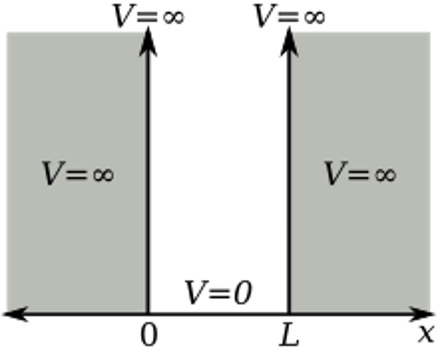
\includegraphics[scale=0.4]{Pot}
\caption{Shéma représentant le potentiel d'un oscillateur harmonique}
\end{figure}
\end{columns}
\end{frame}

%https://fr.wikipedia.org/wiki/Oscillateur_harmonique_quantique#/media/Fichier:Morse-potential-fr.png

\section{L'Hamiltonien}
\begin{frame}
\frametitle{Le potentiel}

L'Hamiltonien de ce système est

\begin{equation}\tag{2}
\hat{H}=-\frac{\hbar^2}{2m}\frac{\partial^2}{\partial x^2}+\hat{V}(x)
\end{equation} 


\end{frame}


\begin{frame}
\frametitle{Le potentiel}


L'Hamiltonien de ce système est

\begin{equation}\tag{2}
\hat{H}=-\frac{\hbar^2}{2m}\frac{\partial^2}{\partial x^2}+k\hat{x}^2
\end{equation} 



\end{frame}

\section{L'Hamiltonien}
\begin{frame}
\frametitle{Équations de Shrodinger indépendante du temps}
Rappelons l'équation de Shrodinger indépendante du temps
\begin{equation}
\hat{H}\Psi(x)=E\Psi(x)
\end{equation}
Les solutions sont de la forme
\begin{equation}
\Psi_{\nu}(x)=N_{\nu}H_{\nu}(y)e^{\frac{-y^2}{2}}
\end{equation}
o\'u $N_{\nu}$ est une constante de normalisation, $H_{\nu}(y)$ est un polynome de Hermite et $y=\frac{x}{\alpha}, \alpha=(\frac{\hbar^2}{mk})^{\frac{1}{4}}$

\end{frame}


\section{L'Hamiltonien}
\begin{frame}
\frametitle{Équations de Shrodinger indépendante du temps}
L'énegie de ces états sont 
\begin{equation}
E_{\nu}=\left(\frac{1}{2}+\nu\right)\hbar\omega
\end{equation}
La différence d'énegie entre les états est constantes
\begin{equation}
E_{\nu+1}-E_{\nu}=\hbar \omega
\end{equation}
\end{frame}



\begin{frame}
\frametitle{Le potentiel}
\begin{figure}
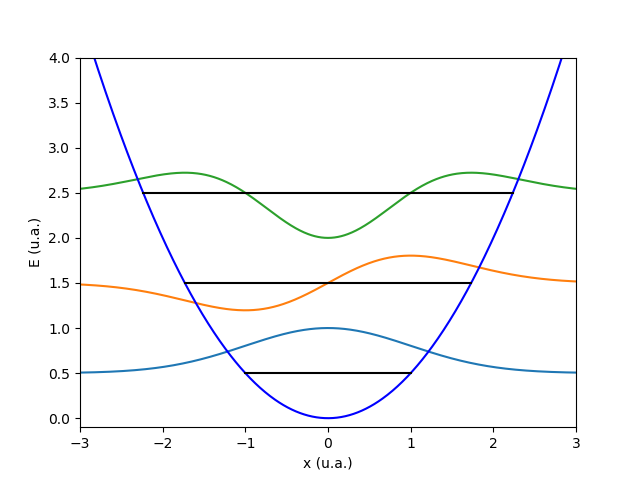
\includegraphics[scale=0.6]{fct_propre}
\caption{Shéma représentant le potentiel d'un oscillateur harmonique}
\end{figure}
\end{frame}

\end{document}



